\section{Cluster}

	\subsection{Le principe}

  Le principe est � partir des variables de calculer la distance entre individus
  et de grouper les individus les plus proches.
  

	\subsection{Temp�rature}

Nous utilisons toujours les donn�es sur la temp�rature.

\begin{knitrout}\footnotesize
\definecolor{shadecolor}{rgb}{0.969, 0.969, 0.969}\color{fgcolor}\begin{kframe}
\begin{alltt}
\hlstd{temp} \hlkwb{<-} \hlkwd{read.csv2}\hlstd{(}\hlstr{"data/temp.csv"}\hlstd{)}
\hlkwd{colnames}\hlstd{(temp)}
\end{alltt}
\begin{verbatim}
##  [1] "Ville"     "Janvier"   "Fevrier"  
##  [4] "Mars"      "Avril"     "Mai"      
##  [7] "Juin"      "Juillet"   "Aout"     
## [10] "Septembre" "Octobre"   "Novembre" 
## [13] "Decembre"  "lati"      "long"
\end{verbatim}
\end{kframe}
\end{knitrout}


	\subsection{Pr�paration des donn�es}

Dans ce cas il faut centrer et r�duire les donn�es pour �viter les probl�mes
de diff�rence d'unit�s.

\begin{knitrout}\footnotesize
\definecolor{shadecolor}{rgb}{0.969, 0.969, 0.969}\color{fgcolor}\begin{kframe}
\begin{alltt}
\hlstd{numerics} \hlkwb{<-} \hlkwd{sapply}\hlstd{(temp,is.numeric)}
\hlkwa{for} \hlstd{(ii} \hlkwa{in} \hlkwd{which}\hlstd{(numerics))}
  \hlstd{temp[[ii]]} \hlkwb{<-} \hlkwd{scale}\hlstd{(temp[[ii]])}
\end{alltt}
\end{kframe}
\end{knitrout}


  \subsection{Peut-on r�sumer les informations ?}

\begin{knitrout}\footnotesize
\definecolor{shadecolor}{rgb}{0.969, 0.969, 0.969}\color{fgcolor}\begin{kframe}
\begin{alltt}
\hlstd{hcpc} \hlkwb{<-} \hlkwd{HCPC}\hlstd{(temp[,}\hlnum{1}\hlopt{:}\hlnum{12}\hlstd{],}\hlkwc{nb.clust} \hlstd{=} \hlnum{3}\hlstd{)}
\end{alltt}


{\ttfamily\noindent\bfseries\color{errorcolor}{\#\# Error in FUN(data[x, , drop = FALSE], ...): 'x' doit �tre num�rique}}\end{kframe}

{\centering 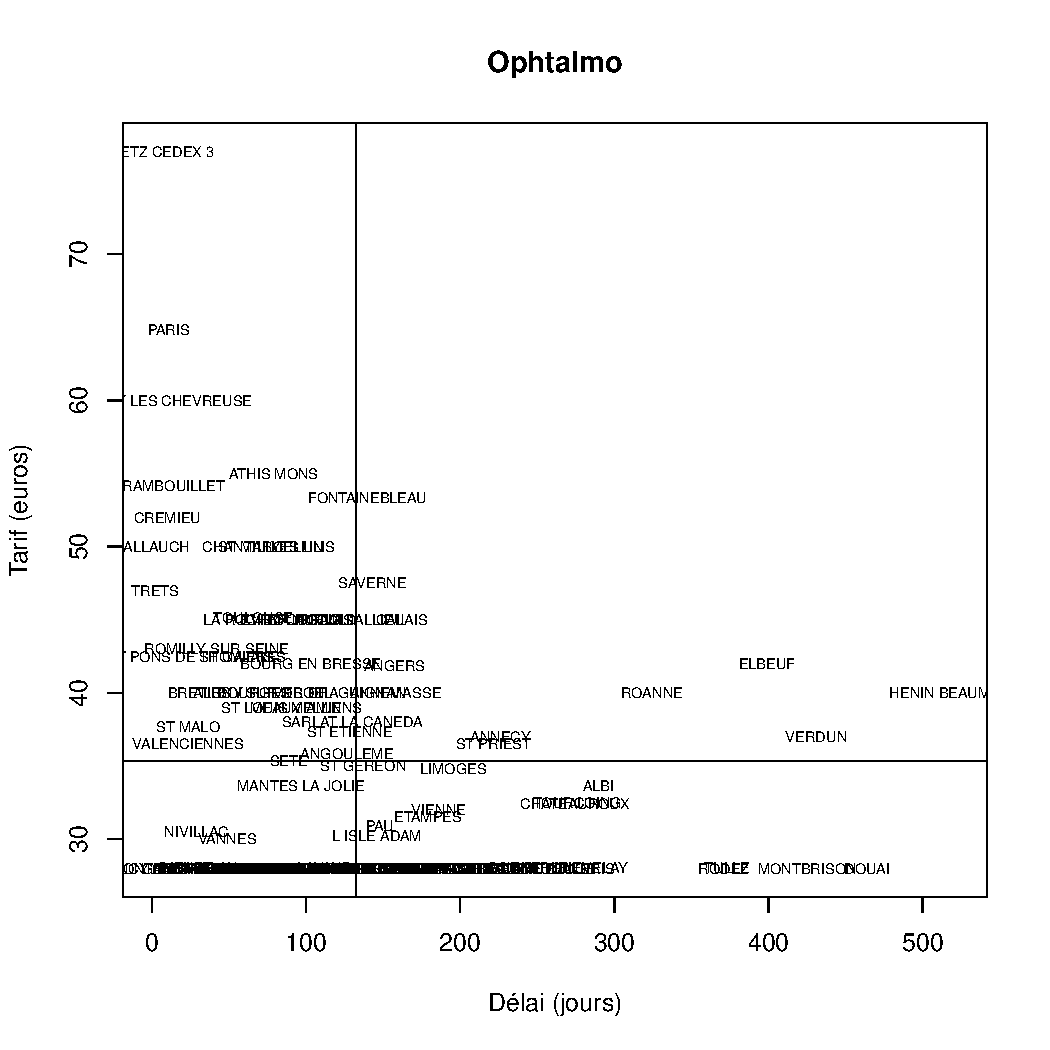
\includegraphics[width=\textwidth]{graphiques/beamer-unnamed-chunk-4-1} 

}



\end{knitrout}



	\subsection{R�sultats}

Nous pouvons voir � la longueur des branches de l'arbre quelles sont les villes
les plus proches les unes des autres. 

Apr�s l'algorithme nous propose une coupure optimale � 3 groupes.



Nous avons 1 groupe qui r�unit les villes les plus au sud, un cluster
qui r�unit les villes de Bretagne au climat peu continental avec 
peu de variations entre les temp�ratures extr�mes et les villes au climat 
plus continental et situ� au nord de la Loire.
  



  
  Le clustering fait partie des m�thodes de \emph{Machine Learning} qui 
  permettent d'analyser les comportements consomnateurs et du profilage
  des individus sur internet.



  


